% file: C01_combined.tex
% author: C. Menges

\documentclass{standalone}
\usepackage{mathtools}
\usepackage{tikz}
\usetikzlibrary{arrows}

\newcommand\setup[0]{
	% grid
	\draw[step=1.0,black,thin] (0,0) grid (10,9);
	% ticks
	\foreach \x in {0,...,9} {
		\node[align=left] at (\x + 0.5,-0.5) {\x};
	}
	% axis
	\draw [thick, |->] (0,-1) -- (9.5,-1);
	\node[align=left] at (9,-1.5) {x};
}

\begin{document}
	% t
	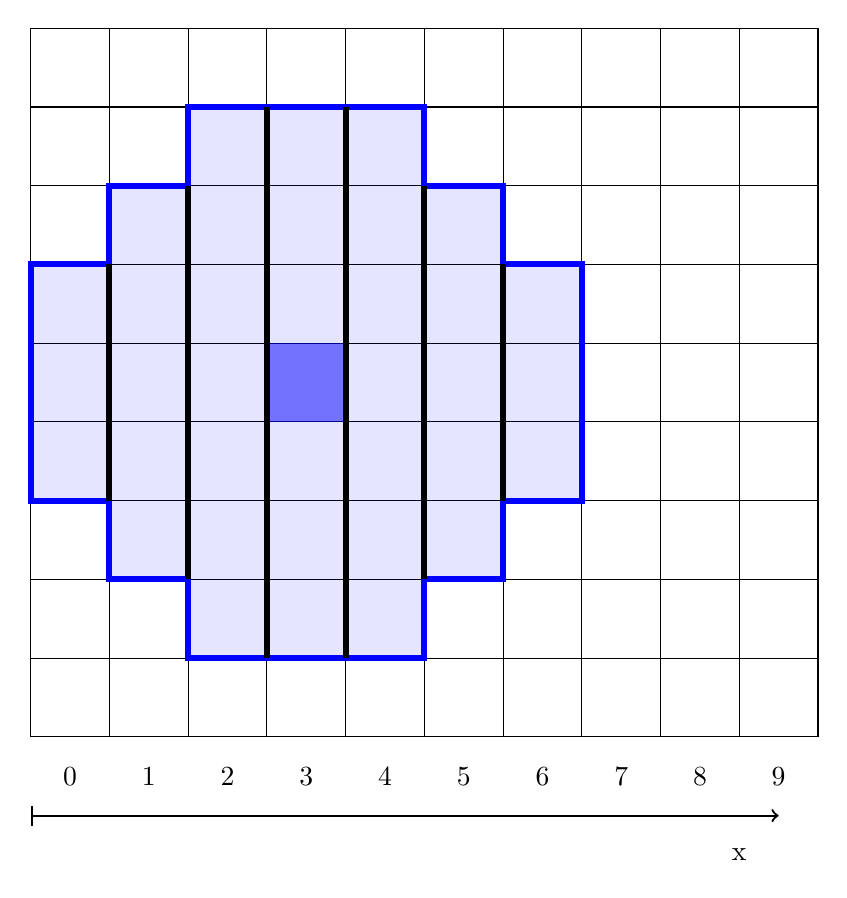
\begin{tikzpicture}[baseline=4cm]
	\setup
	
	% cutoff
	\filldraw [line width=0.75mm, blue, fill opacity=0.1] (0,4) |- (1,6) |- (2,7) |- (3,8) -| (5,7) -| (6,6) -| (7,4) |- (6,3) |- (5,2) |- (4,1) -| (2,2)-| (1,3) -| (0,4);
	
	% base cell
	\fill [blue, opacity=0.5] (3,4) rectangle ++(1,1);
	
	% slices
	\foreach \y [count=\x from 1] in {1,2,3,3,2,1} {
		\draw [black, line width=0.75mm] (\x, 4 - \y) -- (\x, 5+\y);
	}
	\end{tikzpicture}
	
	\begin{huge}
		$\xRightarrow{t \rightarrow t + 1}$
	\end{huge}
	
	% t + 1
	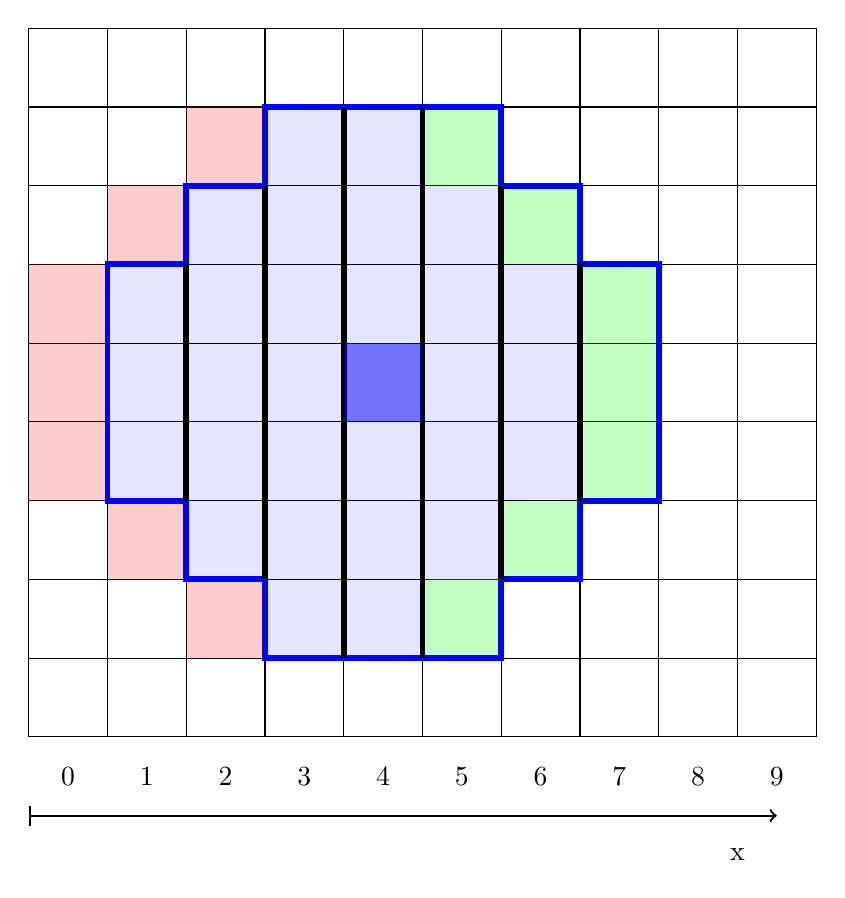
\begin{tikzpicture}[baseline=4cm]
	\setup
	
	\fill [blue, opacity=0.1] (1,4) |- (2,6) |- (3,7) |- (4,8) -| (5,7) -| (6,6) -| (7,4) |- (6,3) |- (5,2) |- (5,1) -| (3,2)-| (2,3) -| (1,4);
	
	% deletions
	\fill [red, opacity=0.2] (1,6) rectangle ++(1,1);
	\fill [red, opacity=0.2] (2,7) rectangle ++(1,1);
	\fill [red, opacity=0.2] (0,3) rectangle ++(1,3);
	\fill [red, opacity=0.2] (1,2) rectangle ++(1,1);
	\fill [red, opacity=0.2] (2,1) rectangle ++(1,1);
	
	% additions
	\fill [green, opacity=0.25] (6,6) rectangle ++(1,1);
	\fill [green, opacity=0.25] (5,7) rectangle ++(1,1);
	\fill [green, opacity=0.25] (7,3) rectangle ++(1,3);
	\fill [green, opacity=0.25] (6,2) rectangle ++(1,1);
	\fill [green, opacity=0.25] (5,1) rectangle ++(1,1);
	
	% cutoff
	\draw [blue, line width=0.75mm] (1,4) |- (2,6) |- (3,7) |- (4,8) -| (6,7) -| (7,6) -| (8,4) |- (7,3) |- (6,2) |- (5,1) -| (3,2)-| (2,3) -| (1,4);
	
	% slices
	\foreach \y [count=\x from 2] in {1,2,3,3,2,1} {
		\draw [black, line width=0.75mm] (\x, 4 - \y) -- (\x, 5+\y);
	}
	
	% base cell
	\fill [blue, opacity=0.5] (4,4) rectangle ++(1,1);
	\end{tikzpicture}
\end{document}